\documentclass[12pt,letterpaper]{article}
\usepackage[margin=1in]{geometry}
\usepackage{amsfonts}
\usepackage{amssymb}
\usepackage{amsthm}
\usepackage{amsmath}
\usepackage{enumerate}

%Here are some user-defined notations
\newcommand{\RR}{\mathbf R}  %bold R
\newcommand{\CC}{\mathbf C}  %bold C
\newcommand{\ZZ}{\mathbf Z}   %bold Z
\newcommand{\QQ}{\mathbf Q}   %bold Q
\newcommand{\rr}{\mathbb R}     %blackboard bold R
\newcommand{\cc}{\mathbb C}    %blackboard bold R
\newcommand{\zz}{\mathbb Z}    %blackboard bold R
\newcommand{\qq}{\mathbb Q}   %blackboard bold Q
\newcommand{\calM}{\mathcal M}  %calligraphic M
\newcommand{\sm}{\setminus} 
\newcommand{\bfa}{\mathbf a}
\newcommand{\bfb}{\mathbf b}
\newcommand{\bfc}{\mathbf c}


\usepackage{tikz}
\usetikzlibrary{positioning}
\usepackage{graphicx}


%Here are some user-defined operators
\newcommand{\re}{\operatorname {Re}}
\newcommand{\im}{\operatorname {Im}}


%These commands deal with theorem-like environments (i.e., italic)
\theoremstyle{plain}
\newtheorem{theorem}{Theorem}[section]
\newtheorem{corollary}[theorem]{Corollary}
\newtheorem{lemma}[theorem]{Lemma}
\newtheorem{conjecture}[theorem]{Conjecture}

%These deal with definition-like environments (i.e., non-italic)
\theoremstyle{definition}
\newtheorem{definition}[theorem]{Definition}
\newtheorem{example}[theorem]{Example}
\newtheorem{remark}[theorem]{Remark}

%your name and date in the header.
\usepackage[us]{datetime} 
\usepackage{fancyhdr}
\pagestyle{fancy}
\lhead{}
\chead{MATH 2710\\ Homework 4}
\rhead{ Your name \\ Oct. 26 2016}
\lfoot{}
\cfoot{}
\rfoot{\thepage}
\renewcommand{\headrulewidth}{0 pt}
\renewcommand{\footrulewidth}{0 pt}
\begin{document}
\ \\
\begin{enumerate}[1.]
\item A sequence of integers $x_1, x_2, x_3,\ldots $ is defined recursively by $x_1=3$, $x_2=7$ and
\[x_k=5x_{k-1}-6x_{k-2}\ \ \text{ for all }k\geq 3\]
Prove by induction that $x_n=2^n+3^{n-1}$ for all positive integers $n$. \\
\ \\
{\bf Solution:}
\begin{proof}
{\bf Base Case:} n=1\\
\ \\
We note the following:
\[ x_1=2^1+3^0=3\]
\ \\
{\bf Induction Hypothesis:} Suppose for $n\leq k$ that 
\[x_k=2^k+3^{k-1}\]
\ \\
We show for $n=k+1$ that 
\[x_{k+1}=2^{k+1}+3^{k}\]
By definition, 
\[x_{k+1}=5x_k-6x_{k-1}\]
Hence by the induction hypothesis, 
\begin{align*}
x_{k+1}&=5x_k-6x_{k-1}\\
&=5(2^{k}+3^{k-1})-6(2^{k-1}+3^{k-2})\\
&=5(2^{k})+5(3^{k-1})-6(2^{k-1})-6(3^{k-2})\\
&=5(2^{k})+5(3^{k-1})-3(2^{k})-2(3^{k-1})\\
&=2^{k+1}+3^{k}\
\end{align*}

\end{proof}
\newpage
\item Prove by induction that a set of $n$ elements contains $2^n$ subsets (including the set itself and $\emptyset$).\\
\ \\
{\bf Solution:} We prove this by induction on the number of elements.
\begin{proof}
{\bf Base Case:} n=1\\
\ \\
Let $A$ be a set with $n=1$ elements, i.e. $A=\{a\}$. Note that $A$ has two subsets: $\{\ \}$ and $\{a\}$.  Hence, our proposition is true for the base case. \\
\ \\
{\bf Induction Hypothesis:} Suppose for $n\leq k$ that a set with $k$ elements has $2^k$ subsets. \\
\ \\
We show for $n=k+1$ that a set with $k+1$ elements has $2^{k+1}$ subsets. Let $A$ be a set with $k+1$ elements. For ease, label the elements with subscripts $1$ through $k+1$, i.e. $A=\{a_1,\ldots a_{k+1}\}$. Now, if $B$ is an arbitrary subset of $A$, then 
\[a_{k+1}\in B\]
or 
\[a_{k+1}\not \in B\]
that is, 
\[B=C\cup \{\}\]
or 
\[B=C\cup \{a_{k+1}\}\]
where $C\subseteq \{a_1,\ldots a_k\}$. By our induction hypothesis, $\{a_1,\ldots a_k\}$ has $2^k$ subsets. Hence, there are $2^k$ subsets of $A$ of the form 
\[C\cup \{\ \}\ \ \ \ \ \text{ where }C\subseteq \{a_1,\ldots a_{k}\}\] and $2^k$ subsets of $A$ of the form 
\[C\cup \{a_{k+1}\}\ \ \ \ \ \text{ where }C\subseteq \{a_1,\ldots a_{k}\}.\]
Since every subset of $A$ is exactly one of these forms we have that $A$ has $2\cdot 2^{k}=2^{k+1}$ subsets. 


\end{proof}
\newpage
\item Prove by induction that if $n$ points lie in a plane and no three are colinear, prove that there are $\frac{1}{2}n(n-1)$ lines joining these points. \\
\ \\
{\bf Example: }
\begin{center}
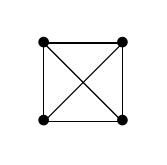
\begin{tikzpicture}
\node at (0,0){$\bullet$};
\node at (1,0){$\bullet$};
\node at (0,1){$\bullet$};
\node at (1,1){$\bullet$};
\draw (1,1)--(0,0) ;
\draw (1,0)--(0,0) ;
\draw (1,1)--(1,0) ;
\draw (0,1)--(0,0) ;
\draw (0,1)--(1,1) ;
\draw (0,1)--(1,0) ;
\end{tikzpicture}
\end{center}
\ \\
{\bf Solution:} We prove this by induction on the number of points in the plane.
\begin{proof}
{\bf Base Case:} n=1\\
\ \\
Suppose that there is one point $p$ in the plane. Obviously, there are $0$ lines connecting $p$ to other points. Hence our proposition is true for the base case.\\
\ \\
{\bf Induction Hypothesis:} Suppose for $n=k$ points in the plane where no three are colinear that there is $\frac{1}{2}k(k-1)$ lines connecting them. \\
\ \\
We show for $n=k+1$ points in the plane where no three are colinear that there are $\frac{1}{2}(k+1)k$ lines connecting them. Suppose there are $k+1$ points in the plane where  no three are colinear. Label them $p_1, \ldots, p_{k+1}$. Consider the points, $p_1, \ldots p_k$. These are $k$ points, in which no three are colinear. By our induction hypothesis, there are $\frac{1}{2}k(k-1)$ lines connecting the points $p_1,\ldots p_k$.  There are $k$ lines connecting $p_{k+1}$ to $p_1,\ldots p_k$ (since there are $k$ points). The total number of lines connecting the points $p_1,\ldots p_{k+1}$ is thus 
\[\frac{1}{2}k(k-1)+k=\frac{k(k-1)+2k}{2}=\frac{k^2+k}{2}=\frac{1}{2}k(k+1)\]
lines connecting the $k+1$ points $p_{1},\ldots p_{k+1}$.\\
\end{proof}
\ \\
{\bf Example: }
\begin{center}
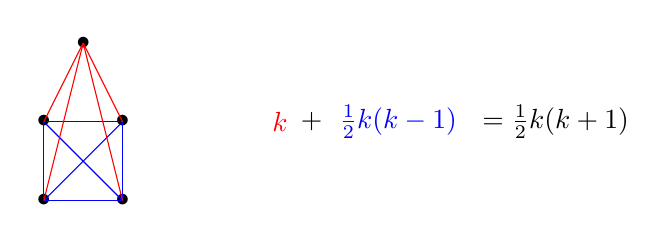
\begin{tikzpicture}
\node at (.5, 2){$\bullet$};
\node at (0,0){$\bullet$};
\node at (1,0){$\bullet$};
\node at (0,1){$\bullet$};
\node at (1,1){$\bullet$};
\draw[blue] (1,1)--(0,0) ;
\draw[blue] (1,0)--(0,0) ;
\draw[blue] (1,1)--(1,0) ;
\draw[blue] (0,1)--(0,0) ;
\draw[blue] (0,1)--(1,1) ;
\draw[blue] (0,1)--(1,0) ;
\draw[red] (.5, 2)--(0,0);
\draw[red] (.5, 2)--(1,1);
\draw[red] (.5, 2)--(0,1);
\draw[red] (.5, 2)--(1,0);
\node[red] at (3,1) {$k$};
\node at (3.40,1){$+$};
\node[blue] at (4.5,1){$\frac{1}{2}k(k-1)$};
\node at (6.5,1){$=\frac{1}{2}k(k+1)$};
\end{tikzpicture}
\end{center}


\newpage

\item Suppose that n chords are drawn in a circle, dividing the circle into different regions.
Prove that every region can be colored one of two colors such that adjacent regions are
different colors. \\
\ \\
{\bf Example: }
\begin{center}
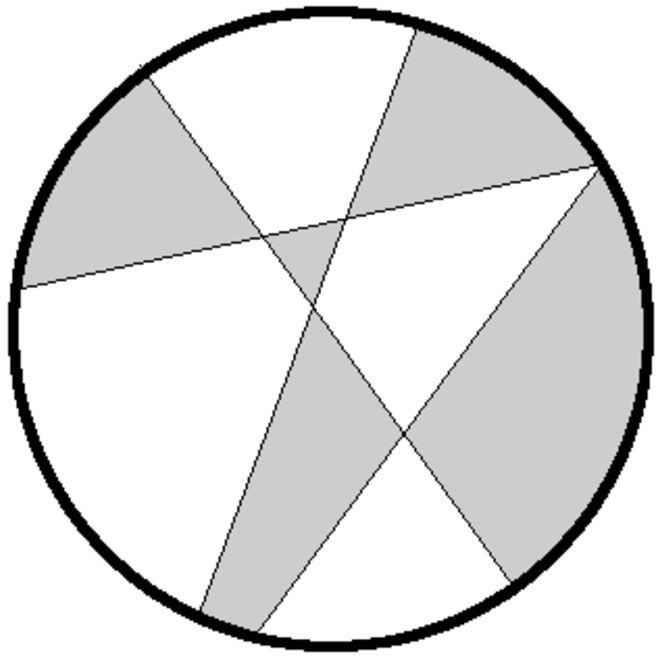
\includegraphics[scale=0.25]{circle}
\end{center}
 
{\bf Solution:} We prove this by induction on the number of chords on the circle.
\begin{proof}
For convenience, we call the property that every region can be colored with one of two colors so that adjacent regions are different colors ``2-colorable". If we have colored the regions with 2 colors so that the adjacent regions are different colors we call that a ``2-coloring". \\
\ \\
{\bf Base Case:} n=1\\
\ \\
One chord cuts a circle into two distinct regions. Obviously, the regions are 2-colorable.\ \\
\ \\
{\bf Induction Hypothesis:} Suppose for $n=k$ chords on the circle that the regions defined by the chords are 2-colorable. \\
\ \\
We show for $n=k+1$ chords that the regions defined by the chords are 2-colorable. Label the chords $\{c_1,\ldots c_{k+1}\}$. The first $k$ chords divide the circle into $n$ regions, label them $A_1, \ldots A_n$. By our induction hypothesis, $A_1, \ldots A_n$ are 2-colorable, i.e. if $A_i$ and $A_j$ (where $i,j\in \{1,\ldots n\}$) are adjacent then $A_i$ and $A_j$ are two different colors. The chords $\{c_1,\ldots c_{k+1}\}$ divide the circle into $m$-regions $B_1, B_2, \ldots, B_m$. Notice, each $B_i$ is contained in some $A_j$. The $k+1$-th chord $c_{k+1}$ divides the circle into two regions $C_1$ and $C_2$. Again, each $B_i$ is contained in either $C_1$ or $C_2$. We now produce a 2-coloring of $B_1, \ldots, B_m$ in a two step process.
\begin{enumerate}[Step 1.]
\item  Given the 2-coloring of $A_1, \ldots A_n$, if $B_i$ is contained in $A_j$ then give it the same color. \\
\ \\
\item Given this coloring of $B_1, \ldots B_m$ to produce a 2-coloring, if $B_i$ is contained in $C_1$ then change the color to the opposite color of $B_i$.\\
 \end{enumerate}
 \newpage
 After Step 1. the regions $B_1, \ldots B_m$ are colored with 2 colors, however two adjacent regions $B_i$ and $B_j$ can be the same color (obviously, this is not a 2-coloring of $B_1, \ldots, B_m$). After Step 2. we have a 2-coloring of $B_1, \ldots B_m$. Since, if two adjacent regions $B_i$ and $B_j$ do not share $c_{k+1}$ as a side, then since they were contained in some $A_\ell$ and $A_d$, they did not share a color after Step 1., changing to the opposite color in Step 2. does not change this. If $B_i$ and $B_j$ shared $c_{k+1}$  as a side, then they were the same color in Step 1. and opposite colors in Step. 2.  
\end{proof}

{\bf Example of Process:}\\
\ \\
\begin{tikzpicture}
\node at (0, 4) {$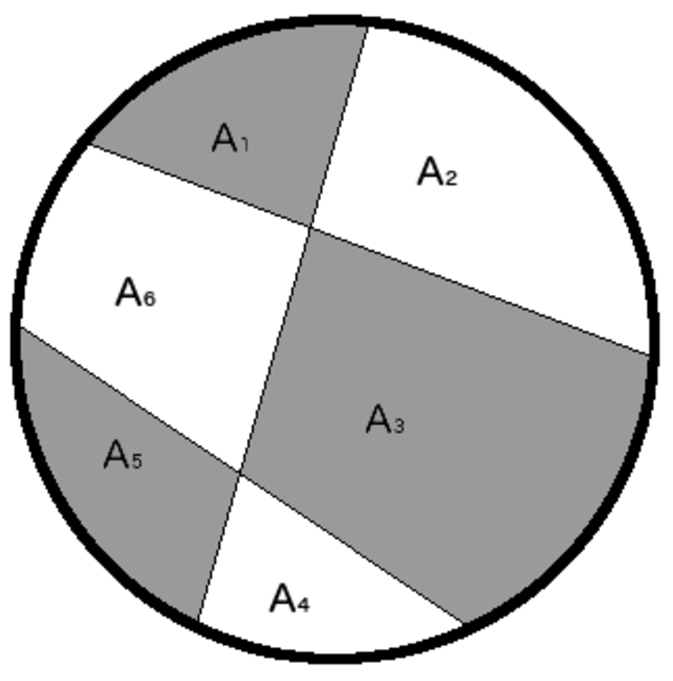
\includegraphics[scale=0.25]{circle1}$};
\node at (0, -2) {k+1 chords};
\node at (0, 2) {2-coloring of k chords};
\node at (0,0) {$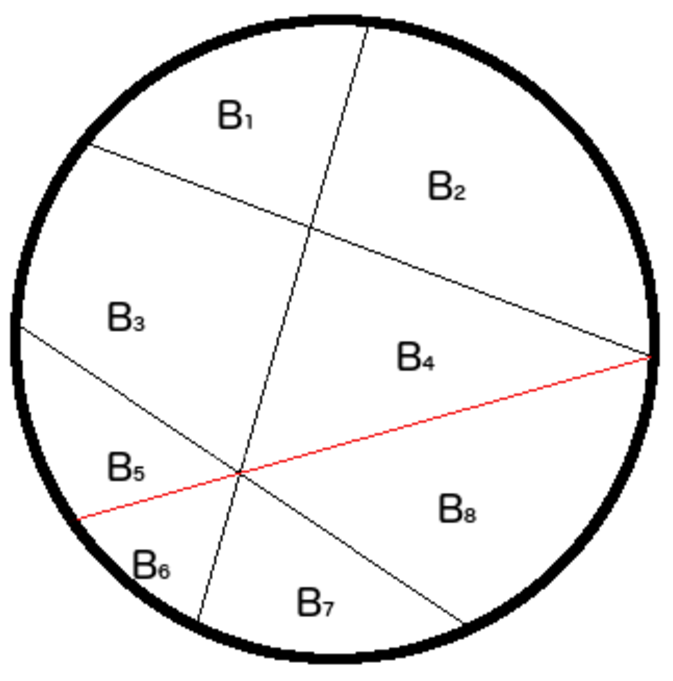
\includegraphics[scale=0.25]{circle2}$}; 
\node at (2, 0) {$\Huge \Rightarrow $};
\node at (4,0) {$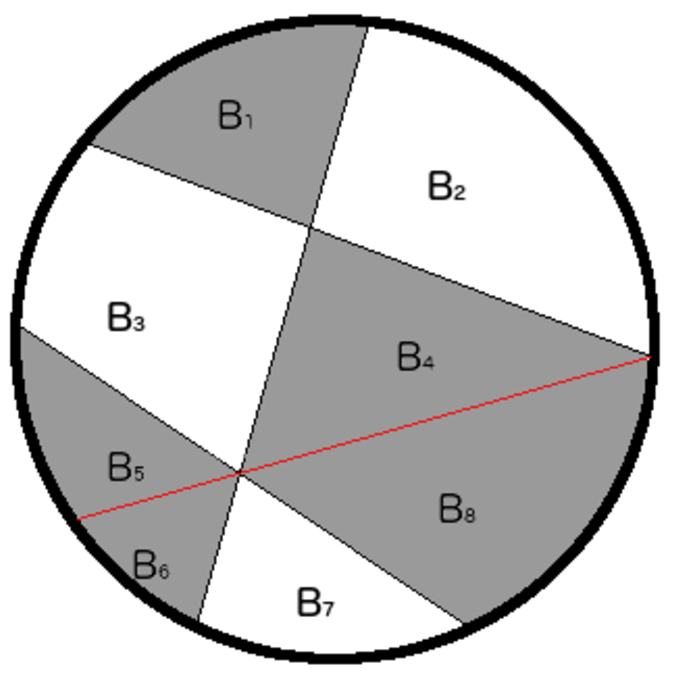
\includegraphics[scale=0.25]{circle3}$}; 
\node at (6, 0) {$\Huge \Rightarrow $};
\node at (8,0) {$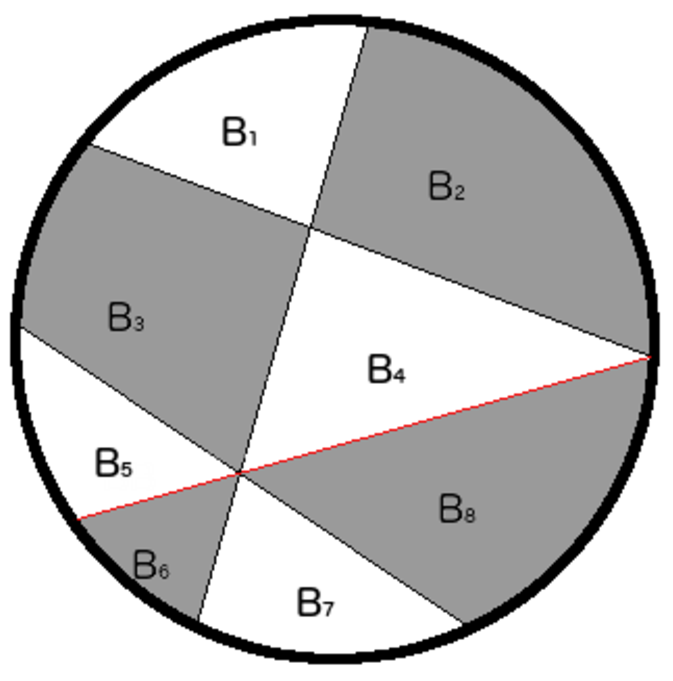
\includegraphics[scale=0.25]{circle4}$}; 
\node at (4, -2) {Step 1.};
\node at (8, -2) {Step 2.};
\end{tikzpicture}
\newpage
\item  Prove that multiplication is a well defined operation on $\mathbb{Q}$.\\
\ \\
{\bf Solution: }
\begin{proof}
Suppose that $\dfrac{a_1}{b_1}=\dfrac{a_2}{b_2}$ and $\dfrac{c_1}{d_1}=\dfrac{c_2}{d_2}$, we need to show that 
\[\frac{a_1c_1}{b_1d_1}=\frac{a_2c_2}{b_2d_2}.\]
In the language of equivalence classes we need to show that if 
\[(a_1,b_1)\sim (a_2, b_2)\ \ \ \ \ \text{ and } \ \ \ \ \ (c_1, d_1)\sim (c_2, d_2)\]
then 
\[(a_1c_1, b_1d_1)\sim (a_2c_2, b_2d_2).\]
This is equivalent to showing that 
\[a_1c_1 b_2 d_2 = a_2 c_2 b_1 d_1.\]
Since $(a_1, b_1)\sim (a_2, b_2)$ we have 
\[a_1b_2=a_2b_1.\]
Likewise, since $(c_1, d_1)\sim (c_2, d_2)$ we have 
\[c_1d_2=c_2d_1.\]
Hence, 
\[
a_1c_1 b_2 d_2 =a_2 b_1 c_1 d_2= a_2 b_1 c_2 d_1.
\]


\end{proof}
\item Prove that $\sqrt{3}$ is irrational. \\
\ \\
{\bf Solution: }
\begin{proof} Suppose there is a rational number $x$ such that $x^2=3$. Let $x=\dfrac{a}{b}$ where $x$ is in lowest terms, i.e. $\gcd(a,b)=1$. Now $\left(\dfrac{a}{b}\right)^2=3$ so we have that $a^2=3 b^2$. Therefore $3\mid a^2 $ and since $3$ is prime we have that $3\mid a$. Hence $a=3c$ for some $c\in \mathbb{Z}$. Therefore $9c^2=3b^2$ and thus $3c^2 = b^2$. It now follows $3\mid b^2$ and hence $3\mid b$. So $3$ is a common divisor of $a$ and $b$, but $\gcd(a,b)=1$. We have a contradiction.
\end{proof}

\end{enumerate}

\end{document}








